
\section{Aplikacja mobilna}
Implementację aplikacji mobilnej rozpocząłem od kreatora, w którym wybrałem opcję pojedynczego Activity. Na początku zaimplementowałem odpowiednie algorytmy skanujące sieci bezprzewodowe w zasięgu. W kolejnym kroku dodałem obsługę urządzenia GPS. Następnie stworzyłem tabelę w bazie danych aplikacji mobilnej z odpowiednią strukturą do przechowywania zebranych obserwacji sieci bezprzewodowych. Na koniec zaimplementowałem prezentację geolokalizacji uzyskanej z aplikacji internetowe oraz możliwość eksportu zebranych obserwacji lokalizacji sieci bezprzewodowych.

\subsection{Uprawnienia na Android}

Począwszy od Androida 6.0 (poziom API 23), użytkownicy przyznają uprawnienia do aplikacji podczas uruchamiania aplikacji, a nie podczas instalowania aplikacji. To podejście usprawnia proces instalacji, ponieważ użytkownik nie musi przyznawać uprawnień podczas instalowania lub aktualizacji. Daje to również użytkownikowi większą kontrolę nad funkcjonalnością aplikacji; Na przykład użytkownik może się zdecydować, czy udostępnić kamerę dostęp do aparatu, ale nie do lokalizacji urządzenia. Dodatkowo użytkownik może cofnąć uprawnienia w dowolnym momencie, przechodząc do ekranu \textit{Ustawienia aplikacji}.\cite{NewPermissionsModelInAndroid60}

Nowy system uprawnień wymaga dodatkowej uwagi twórców aplikacji mobilnych. Zanim

\subsection{Skanowanie sieci bezprzewodowych}
Klasycznym przykładem tego, jak Android został zaprojektowany, jest własnie skanowanie sieci bezprzewodowych. Aby uzyskać obiekty klasy ScanResults. Po pierwsze, musimy uzyskać instancję programu WifiManager. Następnie dziedzicząc po klasie BroadcastReceiver zaimplementować metodę, która dostanie powiadomienie o zakończeniu przetwarzania. Taki asynchroniczny odbiornik — WifiScanReceiver — rejestrujemy z parametrem SCAN\_RESULTS\_AVAILABLE\_ACTION i wreszcie rozpocząć skanowanie przez metodę startScan() na instancji WifiManager.

\begin{minted}[breaklines=true]{java}
wifi_manager = (WifiManager) getApplicationContext().getSystemService(Context.WIFI_SERVICE);
wifi_scan_reciever = new WifiScanReceiver();
registerReceiver(wifi_scan_reciever, new IntentFilter(WifiManager.SCAN_RESULTS_AVAILABLE_ACTION));
wifi_manager.startScan();
\end{minted}

W Androidzie nie ma możliwości zparametryzowania, że chcemy uzyskiwać wyniki o zeskanowanych sieciach w sposób ciągły. Musimy więc w naszym WifiScanReceiver zlecić ponowne skanowanie zaraz po otrzymaniu wyniku ostatniego skanowania. Warto w tym miejscu dopisać sprawdzenie, czy współrzędne geograficzne ostatnio zapisane z urządzenia GPS są aktualne. W przeciwnym przypadku nie zapisywać informacji o lokalizacji ze względu na nieaktualność posiadanych współrzędnych.

\begin{minted}[breaklines=true]{java}
private class WifiScanReceiver extends BroadcastReceiver {
    public void onReceive(Context context, Intent intent) {
        wifi_manager.startScan();
        if( last_location != null && ( (1000*10) > Calendar.getInstance().getTime().getTime() - last_location.getTime())){
            List<ScanResult> wifiScanList = wifi_manager.getScanResults();
            for (ScanResult wifi : wifiScanList) {
                if( wifi.SSID.contains("_nomap") || wifi.SSID.contains("_optout") ){
                    wifiScanList.remove(wifi);
\end{minted}
W powyższym kodzie źródłowym widzimy usuwanie wyników zeskanowanych sieci z określonymi frazami w nazwie sieci. Wiąże się to z faktem, że firma Google zaproponowała dopisywanie do końca nazwy sieci frazę \_nomap (z ang. nie mapuj), aby ich produkty i rozwiązania nie zbierały informacji o lokalizacji danych sieci bezprzewodowych.\cite{GoogleNomap} Dodatkowego zamieszania dorzuciła firma Microsoft, gdzie dla swoich rozwiązań zaproponowali frazę \_optout (z ang. wypisz mnie).\cite{MicrosoftOptout}

\subsubsection{Problem z określeniem kierunku sygnału}
Nie jest możliwym stwierdzenie, z jakiego kierunku przyszedł sygnał sieci bezprzewodowej w przypadku, gdy urządzenie posiada jedną kartę sieciową i posiadamy tylko jedną informację z lokalizacją i sygnałem sieci. Powoduje to, że zbieranie informacji o lokalizacjach sieci bezprzewodowych jest skazane na dużą niedokładność. Dla algorytmów bardzo prymitywnych spowoduje to umiejscowienie wszystkich sieci bezprzewodowych na pozycji telefonu np. na środku ulicy lub na chodniku. Bardzo dobrze to widać na Rysunku \ref{fig:poor-scan-result}

\begin{figure}[h!]
  \centering
    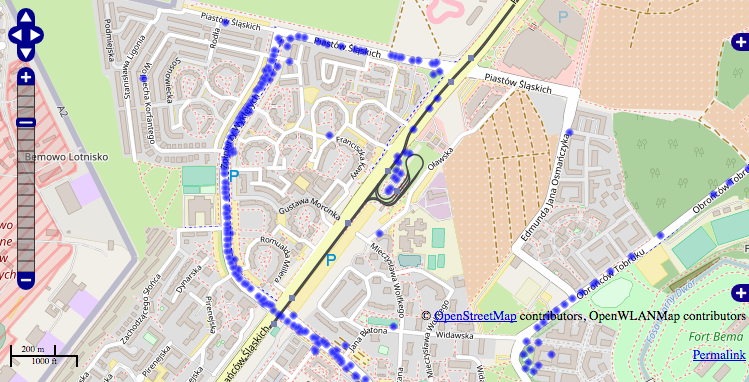
\includegraphics[width=10cm]{images/poor-scan-result}
  \caption{Prezentacja lokalizacji sieci bezprzewodowych na mapie - algorytm primitywny}
  \label{fig:poor-scan-result}
\end{figure}

Rozwiązanie lepsze, ale droższe, to użycie kilku urządzeń, najlepiej z antenami kierunkowymi, dzięki czemu moglibyśmy stwierdzić czy stacja bazowa znajduje się po lewej stronie ulicy, czy po prawej na podstawie różnicy w sile sygnału. Dzięki technologii MIMO można określić, z którego kierunku przyszedł sygnał wykorzystując jedno urządzenie. Ze względu na denormalizację obserwacji sieci bezprzewodowych jesteśmy w stanie estymować kierunek, z którego przyszedł sygnał o ile mamy kilka zarejestrowanych skanów z różnymi siłami i lokalizacjami.

\subsection{Określanie lokalizacji urządzenia}
Do obsługi lokalizacji urządzenia poprzez GPS wykorzystałem bibliotekę — SmartLocation. Użycie prostego interfejsu biblioteki zaoszczędziło dużo czasu, który musiałbym poświęcić na zapoznawanie się z dokumentacją klas i interfejsów dotyczących nawigacji w Androidzie.

\begin{minted}[breaklines=true]{java}
public void startGpsListener(){
    SmartLocation.with(this).location()
      .config(LocationParams.NAVIGATION).continuous()
      .start(gps_location_listener);
}
private class GpsLocationListener implements OnLocationUpdatedListener {
    @Override
    public void onLocationUpdated(Location location) {
        last_location = location;
    }
}
\end{minted}

Sam proces uzyskania informacji o lokalizacji urządzenia jest asynchroniczny. Aby zniwelować efekt asynchroniczności, utworzyłem lokalną zmienną w ramach widoku, do której zapisuję ostatnią otrzymaną pozycję z SmartLocation. Do uzyskania najdokładniejszej pozycji skorzystałem z funkcji trybu nawigacji (z ang. navigate) z parametrem pracy ciągłej (z ang. continious). Trzeba pamiętać, że takie ustawienie jest niekorzystne dla czasu pracy na baterii, ale gwarantuje to najświeższą informację o współrzędnych urządzenia.

\subsection{Baza danych}
Teraz gdy już mamy wyniki skanowania sieci bezprzewodowych i lokalizację urządzenia, to jesteśmy w stanie zapisać wyniki do bazy danych aplikacji mobilnej — aby potem przesłać do aplikacji internetowej — dla lepszej precyzji określania lokalizacji sieci bezprzewodowych, a tym samym użytkownika.

Wybrałem bibliotekę ActiveAndroid jako ORM ze względu na swoje podobieństwo do ActiveRecord ze środowiska języka programowania Ruby oraz ze względu na użycie bazy SQLite, która jest popularnym rozwiązaniem do przechowywania danych na Androidzie. Stosując się do dobrych praktych twórców tej biblioteki, umieściłem tworzenie obserwacji w transakcji:

\begin{minted}[breaklines=true]{java}
ActiveAndroid.beginTransaction();
try {
    for (ScanResult wifi : wifiScanList) {
        WifiObservation wifiObservation = new WifiObservation(wifi, last_location);
        wifiObservation.save();
    }
    ActiveAndroid.setTransactionSuccessful();
} finally {
    ActiveAndroid.endTransaction();
}
\end{minted}

Po raz kolejny podjąłem decyzję o denormalizacji danych. Dane takie będą zajmować więcej miejsca, ale umożliwią na dokładniejsze lokalizowanie miejsca, w którym jest umiejscowiony punkt dostępu. Wszystkie dane będą zapisane w pojedynczej tabeli.

\begin{table}
\caption{Kolumny i typy przechowywania danych wraz z ich znaczeniem w aplikacji mobilnej}
\label{table:mobiledbscheme}
\begin{tabular} { |l|l|p{7cm}|  }
\hline
Typ & Nazwa & Znaczenie (opcjonalne) \\
\hline
\hline
String & ssid & \\
\hline
String & bssid & \\
\hline
int & signal\_level & Wykryty poziom sygnału w dBm, znany również jako RSSI.\cite{scanResultAndroidDocs} \\
\hline
String & capabilities & Opisuje schematy uwierzytelniania, zarządzania kluczami i szyfrowania obsługiwane przez punkt dostępu.\cite{scanResultAndroidDocs} \\
\hline
Date & observed\_at & Data i czas o sieć została zeskanowana \\
\hline
int & channel\_frequency & Częstotliwość zeskanowanej sieci \\
\hline
double & latitude & Szerokość geograficzna pozycji, w której sieć zeskanowano \\
\hline
double & longitude & Wysokość geograficzna pozycji, w której sieć zeskanowano \\
\hline
Date & geolocated\_at & Data i czas otrzymania informacji o współrzędnych geograficznych urządzenia \\
\hline
float & geolocation\_accuracy & Dokładność współrzędnych geograficznych pozycji w któ®ej sieć zeskanowano \\
\hline
boolean & is\_exported & Informacja o tym, czy sieć została wyeksportowana do aplikacji internetowej \\
\hline
\end{tabular}
\end{table}

Konstruktor klasy WifiObservation przyjmujący zeskanowaną sieć oraz ostatnią lokalizację zaimplementowałem następująco:
\begin{minted}[breaklines=true]{java}
public WifiObservation(ScanResult scanResult, Location location){
    super();
    this.ssid = scanResult.SSID;
    this.bssid = scanResult.BSSID;
    this.signal_level = scanResult.level;
    this.capabilities = scanResult.capabilities;
    this.channel_frequency = scanResult.frequency;

    this.observed_at = new Date();

    this.latitude = location.getLatitude();
    this.longitude = location.getLongitude();
    this.geolocated_at = new Date(location.getTime());
    this.geolocation_accuracy = location.getAccuracy();

    this.is_exported = false;
}
\end{minted}

\subsection{Określenie identyfikatora urządzenia}
Przy zbieraniu informacji o lokalizacjach sieci bezprzewodowych chciałem, aby dane obserwacje były oznaczone, przez jakie urządzenie zostały zaimportowane. Stosując zalecane rozwiązanie, napisałem metodę, która przy pierwszym uruchomieniu generuje unikalny identyfikator i zapisuje go w przestrzeni ustawień aplikacji mobilnej. Każde następne uruchomienie, pobierze ten wcześniej wygenerowany identyfikator.\cite{SOSharedPrefreneces}
\begin{minted}[breaklines=true]{java}
public String getUniqueDeviceId(){
    SharedPreferences sharedPref = getPreferences(Context.MODE_PRIVATE);
    String device_id = sharedPref.getString(preferenceUniqueIdKey, null);
    if(device_id == null){
        SharedPreferences.Editor editor = sharedPref.edit();
        device_id = UUID.randomUUID().toString();
        editor.putString(preferenceUniqueIdKey, device_id);
        editor.apply();
    }
    return device_id;
}
\end{minted}

\subsection{Prezentacja danych — mapa}
Finalną częścią aplikacji mobilnej była prezentacja danych oraz zaimplementowanie algorytmów do zbadania tych danych. Wykorzystałem do tego problemu wczęśniej wspomnianą bibliotekę leaflet. Stworzyłem Androidową kontrolkę WebView do której poprzez odpowiedni interfejs JavaScriptowy przekazałem aktualną pozycję z urządzenia GPS oraz sieci zeskanowane w zasięgu smartfonu. Ze względu na różnice w interfejsie klasy WebView, na przestrzeni lat zmienił się sposób uruchamiana JavaScriptu. Zaimplementowałem odpowiednie sprawdzenie, aby uzyskać zgodność ze starym oraz nowym interfejsem klasy WebView.

\begin{minted}[breaklines=true]{java}
public void runJavascript(String code){
    if (android.os.Build.VERSION.SDK_INT >= android.os.Build.VERSION_CODES.KITKAT) {
        webView.evaluateJavascript(code, null);
    } else {
        webView.loadUrl("javascript:("+code+");");
    }
}
\end{minted}

Ze względu na fakt, że wszystkie operacje są wykonywane w logice widoku, każde uśpienie aplikacji wstrzymywało pomiary i urządzenie GPS. Dodałem odpowiednią flagę do okna aplikacji, która poinformowała system o tym, żeby nie usypiać urządzenia w trakcie działania tej aplikacji.

\begin{minted}[breaklines=true]{java}
protected void onCreate(Bundle savedInstanceState) {
    super.onCreate(savedInstanceState);
    webView = new WebView(this);
    setContentView(webView);
    getWindow().addFlags(
      WindowManager.LayoutParams.FLAG_KEEP_SCREEN_ON);
    // ...
}
\end{minted}

Przy tworzeniu mapy, okazało się, że aplikacja internetowa nie posiadała odpowiednich nagłówków pozwalających na uruchamianie zapytań z innych domen. Rozwiązaniem tego problemu było dodanie odpowiednich nagłówków standardu Cross-Origin Resource Sharing. W przypadku aplikacji Ruby On Rails globalnie ten problem rozwiązałem przez import biblioteki rack-cors i konfigurację serwera aplikacji przy uruchamianiu:

\begin{minted}[breaklines=true]{ruby}
module RailsAppStartingTemplate
  class Application < Rails::Application
    # ...
    config.middleware.insert_before 0, Rack::Cors do
      allow do
        origins '*'
        resource '*', :headers => :any, :methods => [:get, :post, :options]
      end
    end
    # ...
  end
end
\end{minted}

Samą prezentację oraz monitorowanie parametrów geolokacji rozwiązałem poprzez zapisanie ilości wykonanych geolokalizacji, zsumowanie wszystkich deklarowanych precyzji geolokalizacji (aby otrzymać średnią arytmetyczną) i zmierzenie otrzymanej lokalizacji w porównaniu do obecnej lokalizacji podanej przez GPS i zsumowanie jej do poprzednich wartości (dla średniej arytmetycznej).

\begin{minted}[breaklines=true]{javascript}
geowifiTimes += 1;
geowifiAccuracy += parseFloat(data.accuracy || 0)
geowifiMeasuredAccuracy += distance(gpsMarker.getLatLng().lat, gpsMarker.getLatLng().lng, data.location.lat, data.location.lng)
wifiMarker.setLatLng([data.location.lat, data.location.lng]);
fitMarkersIntoScreen();
\end{minted}

Dzięki temu, że interfejs geolokalizacji mojej aplikacji internetowej, działa zgodnie ze specyfikacją interfejsu produkty Mapy firmy Google w części geolokalizacji na podstawie sieci bezprzewodowych, to mogłem dodać bardzo niskim kosztem ich serwer geolokacji i zmierzyć jego parametry. Dla rozróżnienia, nadałem mojej aplikacji nazwę geowifi. Obliczenie i prezentacja danych została zaimplementowana następująco:
\begin{minted}[breaklines=true]{javascript}
this._div.innerHTML = '<strong>Średni czas:</strong>';
this._div.innerHTML += '<br>GeoWifi: ' + (  (((new Date()) - timeStart)/1000) / geowifiTimes ).toFixed(3) + ' s';
this._div.innerHTML += '<br>Google: ' + (  (((new Date()) - timeStart)/1000) / googleTimes ).toFixed(3) + ' s';

this._div.innerHTML += '<br><strong>Średnia deklarowana precyzja:</strong>';
this._div.innerHTML += '<br>GeoWifi: ' + parseInt(  geowifiAccuracy / geowifiTimes ) + ' m';
this._div.innerHTML += '<br>Google: ' + parseInt(  googleAccuracy / googleTimes ) + ' m';

this._div.innerHTML += '<br><strong>Średnia zmierzona precyzja:</strong>';
this._div.innerHTML += '<br>GeoWifi: ' + parseInt(  geowifiMeasuredAccuracy / geowifiTimes ) + ' m';
this._div.innerHTML += '<br>Google: ' + parseInt(  googleMeasuredAccuracy / googleTimes ) + ' m';

this._div.innerHTML += '<br><strong>Liczba geolokacji:</strong>';
this._div.innerHTML += '<br>GeoWifi: ' + parseInt( geowifiTimes );
this._div.innerHTML += '<br>Google: ' + parseInt(  googleTimes );
\end{minted}


\section{Badanie i wnioski}
Na tym etapie pracy zauważyłem już, że zaimportowane dane z publicznych baz danych były bardzo ograniczone. Dla obszaru Warszawy zaimportowanych zostało mniej niż \textbf{200 tysięcy unikalnych} pozycji sieci bezprzewodowych, co w porównaniu z szacowanymi \textbf{944 012} z części teoretycznej, zapowiadało porażkę. Dlatego dla obszarów mojego zamieszkania i miejsca pracy wykonałem kilka przejść z aplikacją i wyeksportowałem informacje o lokalizacjach sieci bezprzewodowych. Szacuję , że zagęszczenie w tych lokalizacjach zwiększyło się przynajmniej dwukrotnie.

\subsection{Pomiar zagęszczenia sieci bezprzewodowych na terenie Warszawy}
Pomiar zagęszczenia w Warszawie oparłem na 3 próbkach. Dwie wybrane ręcznie ze względu na ograniczony zestaw informacji o lokalizacjach sieci bezprzewodowych oraz jeden wybrany losowo. Kod źródłowy obliczający gęstość sieci na km\textsuperscript{2} wyglądał następująco:

\begin{minted}[breaklines=true]{ruby}
distance = 0.5
warsaw_spire_plac_europejski_1 = [52.232175, 20.984187]
losowy = [52.273075, 20.974593]
zeromskiego_1 = [ 52.275371, 20.960779]

[
  WifiPosition.within_bounding_box(
    Geocoder::Calculations.bounding_box(losowy, distance)).length,
  WifiPosition.within_bounding_box(
    Geocoder::Calculations.bounding_box(
    warsaw_spire_plac_europejski_1, distance)).length,
  WifiPosition.within_bounding_box(
    Geocoder::Calculations.bounding_box(zeromskiego_1, distance)).length
]
\end{minted}

\begin{table}
\caption{Wyniki pomiaru gęstości sieci bezprzewodowych}
\label{table:densityResult}
\begin{tabular} { |l|l|  }
\hline
Lokalizacja & Ilość bezprzewodowych sieci na km\textsuperscript{2} \\
\hline
\hline
Losowy punkt & 536 \\
Plac Europejski 1 & 993 \\
Żeromskiego 1 & 1129 \\
\hline
\end{tabular}
\end{table}

Wartości z Tablicy \ref{table:densityResult} potwierdzają, że Warszawa posiada odpowiednią infrastrukturę sieci bezprzewodowych, aby nawigować po niej przy użyciu tylko lokalizacji sieci bezprzewodowych. Szacuję że dla rejonów centrum Warszawy powinniśmy zobaczyć wartości powyżej 3 lub 4 tysięcy. Jednak zeskanowanie lokalizacji sieci bezprzewodowych na obszarze kilometra kwadratowego to kosztowna operacja i podejrzewam to za główny powód niedokładności publicznych zbiorów danych.

\subsection{Pomiar precyzji geolokalizacji}
W kwestii precyzji wyniki nie były bardzo satysfakcjonujące, co widać na Rysunku \ref{fig:mapResult} Zmierzona precyzja geolokalizacji nie osiągnęła minimalnej wymaganej określonej w tezie. Nie oznacza to, że nie można nawigować przy użyciu lokalizacji sieci bezprzewodowych. Oznacza to jedynie, że nie jest ona odpowiednią konkurencją dla urządzeń GPS. Osiągnięte wyniki jednak nie są bardzo złe. W przy średniej zmierzonej precyzji osiągnięto 50,513 metra dla sposobu przedstawionego w tej pracy. Oraz 55,074 dla platformy Google Maps. Zauważalna jest duża różnica w stosunku do deklarowanej precyzji przez obydwie platformy. Odpowiednio 243,948 metra dla aplikacji internetowej (geowifi) oraz 72,096 dla platformy Google. W pomiarze wystąpiły pełne 73 cykle geolokalizacji.

\begin{figure}[h]
  \centering
    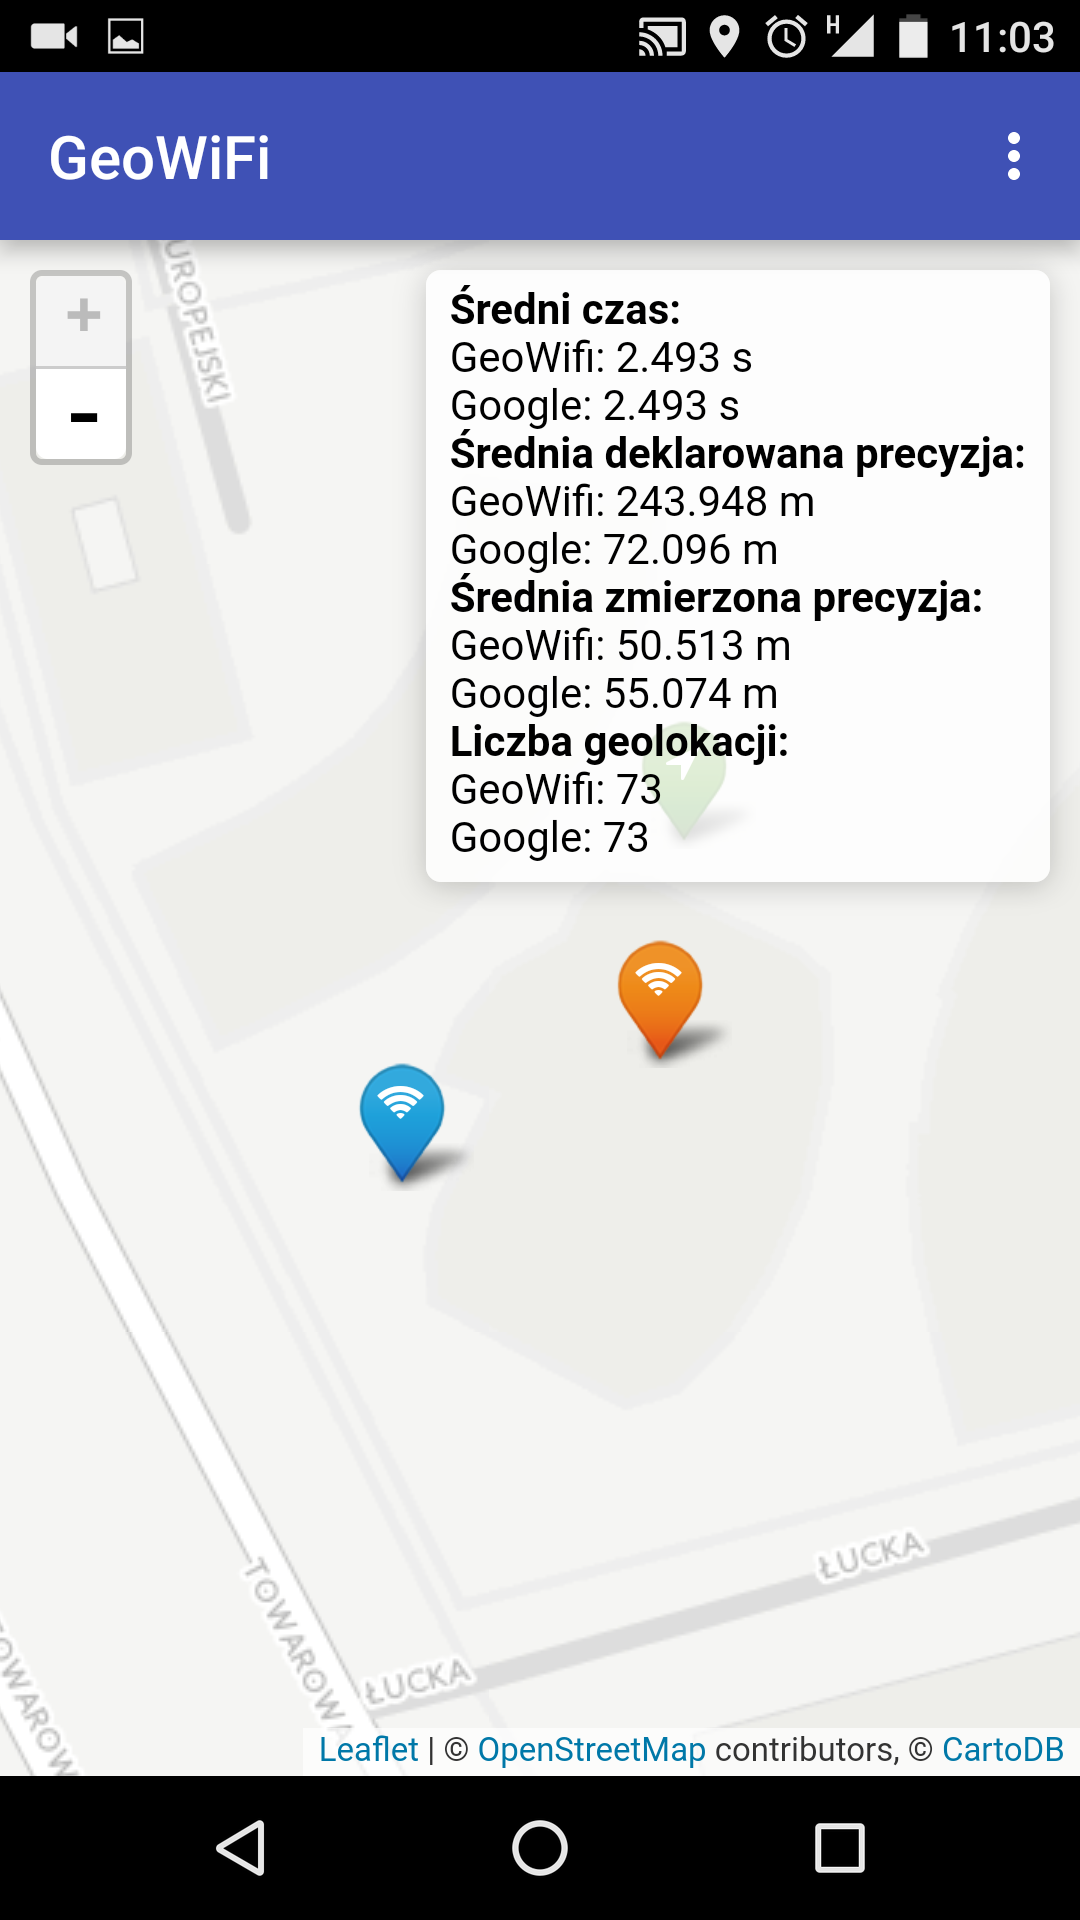
\includegraphics[width=8cm]{images/map-result}
  \caption{Zrzut ekranu z aplikacji mobilnej na koniec pomiaru precyzji i szybkości geolokalizacji}
  \label{fig:mapResult}
\end{figure}

\subsection{Pomiar szybkości geolokalizacji}
W każdym cyklu tym najwięcej czasu zajmowało zeskanowanie sieci bezprzewodowych przez urządzenie. Na badanym urządzeniu udało się osiągnąć wynik 2.493 sekund na pełen cykl geolokalizacji.(Rysunek \ref{fig:mapResult}) Jest to zadowalający wynik, jednak w aplikacjach nawigacyjnych podejrzewam, że trzeba byłoby kompensować tak niską częstotliwość odświeżania pozycji, szacunkami na podstawie kierunku i prędkości urządzenia.

\subsection{Wnioski}
Praca ta dowodzi, że Warszawa jest odpowiednio rozwiniętym i nowoczesnym miastem. Urządzenia są w stanie określać geolokalizację w odpowiedniej częstotliwości. Niestety jednak precyzja pozostawia wiele do życzenia. Możliwe jest stosowanie takiej geolokalizacji do urządzeń, w których niepotrzebna jest precyzyjna lokalizacja, a zmniejszone koszty zużycia baterii dla geolokalizowania są pożądane. Takie urządzenia i ich zastosowania to mogą być krokomierze, systemy lokalizowania skradzionych przedmiotów — w tych przypadkach, geolokalizacja na podstawie sieci bezprzewodowych może mieć nawet lepsze efekty niż urządzenia GPS ze względu na fakt, że technologia GPS wymaga dostępu do tzw. otwartego nieba.

Podsumowując: aby wykorzystać rozwiązanie geolokalizowania na podstawie sieci bezprzewodowych, trzeba opracować algorytmy, o lepszej precyzji i utworzyć dokładniejsze bazy danych o lokalizacjach. Ewentualnie można wykorzystać to rozwiązanie do określania lokalizacji z precyzją rzędu ponad 50 metrów.
